
\documentclass[12pt,a4paper]{article}
\usepackage{times}
\usepackage{durhampaper}
\usepackage{harvard}
\usepackage{graphicx}

\citationmode{abbr}
\bibliographystyle{agsm}

\title{Implementation and Analysis of an Elliptic Curve Cryptography System}
%\author{} % leave; your name goes into \student{}
\student{T. Butterfield}
\supervisor{M. Bordewich}
\degree{BSc Computer Science}

\date{\today}

\begin{document}

\maketitle

\begin{abstract}
Do not cite references in the abstract.

This section should not be longer than half of a page, and having no more than one or two sentences under each heading is advised.

\paragraph{Background} -
Diffie-Hellman, RSA, ...

\paragraph{Aims} -
The aim of this project was to create a working Elliptic Curve Cryptography system 
and to analyse that system in terms of security and efficiency. 

\paragraph{Method} -
Euclid's extended algorithm, point addition, point multiplication, ...

\paragraph{Results} -
Cannot discover information about private key, enables secure communication

\paragraph{Conclusions} -
Strength of ECC, smaller key size than RSA, much more suitable for mobile devices

\end{abstract}


\begin{keywords}
Elliptic Curve Cryptography (ECC), Elliptic Curve Diffie-Hellman (ECDH), Elliptic Curve Digital Signature Algorithm (ECDSA), 
Safe Curves, User Interface (UI)
\end{keywords}


\section{Introduction}\noindent
There were a total of nine objectives for this project, split equally into three sections: basic, intermediate, and advanced. 

The first basic objective was to create a basic working ECC system which computed the essential functions required. 
The second and third basic objectives were to create a client application that can conduct ECDH over a network connection, 
and to create a UI allowing a user to easily make use of the system and to decide what level of complexity is revealed to them. 

The intermediate objectives revolved around improving the functionality and security of the system, 
with the first objective being to add secure random private key generation to the system. 
The other intermediate objectives were to implement the ECDSA and to enable the exchange of secure signed files via the UI. 

The first advanced objective was to make improvements to the UI and to reveal the workings of the system. 
The penultimate objective was to analyse the code for efficiency, including how the time required scales with the curve and key size, 
making any necessary changes to the system to improve the efficiency. 
The final objective was to analyse the code for vulnerabilities, such as side-channel attacks, and to fix any such weaknesses. 


\section{Related Work}\noindent
Cryptography is the study of mathematical systems for solving two kinds of security problems: privacy and authentication \cite{1055638}. 
A privacy system prevents the extraction of information by unauthorised parties from messages transmitted over a public channel, assuring it is read only by the intended recipient. 
An authentication system prevents the unauthorised injection of messages into a public channel, assuring the legitimacy of the sender. 
Diffie \& Hellman \citeyear{1055638} proposed that it was possible to develop systems in which two parties communicating solely over a public channel and using only publicly known techniques could create a secure connection. 
This was the first public discovery of public-key cryptography.

Diffie and Hellman presented the concept of a public-key cryptosystem but not any practical implementation of such a system. 
So in 1978, Rivest, Shamir, and Adleman presented a new encryption method which did just that, it was the first public implementation of public-key cryptography. 
This method had the novel property that publicly revealing an encryption key did not thereby reveal the corresponding decryption key \cite{10.1145/359340.359342}. 
This is known as RSA public-key cryptography. 

Miller \citeyear{10.1007/3-540-39799-X_31} and Koblitz \citeyear{koblitz1987elliptic} discussed an analogue of the Diffie-Hellman key exchange protocol based on elliptic curves over finite fields which used the multiplicative group of a finite field. 
The advantage of this system was that it appeared to be immune from attacks of the style of \cite{10.1007/3-540-39799-X_31,4568001}. 
This was the invention of Elliptic Curve Cryptography. 

Whilst the \emph{Elliptic Curve Discrete Logarithm Problem} is difficult to solve on classical computers \cite{hankerson2003guide}, 
there is a gap between ECDLP difficulty and ECC security \cite{bernstein2013safecurves}. 
In 2010, it was discovered that Sony had made a basic and critical mistake in the implementation of their Elliptic Curve Cryptosystem. 
As discussed in section \ref{Signature Generation}, as part of the Signature Generation stage of the ECDSA, a random integer $k$ is generated and used, 
it is imperative that $k$ is truly random and not predictable in any way. 
However, Sony wrote their own software which used a constant number for each signature. 
This allowed the computation of their private key, from the public key, using simple algebra \cite{hotz2010console}.


\section{Solution}\noindent
This section presents the solutions to the problems in detail. 
Included here are details of the specification and design (Section \ref{Specification}), 
an outline of the implementation issues faced (Section \ref{Implementation}), 
a description of the tools used (Section \ref{Tools}), 
as well as the verification and validation of the components (Section \ref{Verification}), 
and finally a discussion of the testing of the system (Section \ref{Testing}). 

\subsection{Architecture and Design}\noindent \label{Specification}
At a high level, my system is a client-server network designed to allow 
multiple instances of a client program to connect to a single server program. 
The clients can communicate with each other, via the server, using end-to-end ECC encryption. 
In the description and explanation of my system I will personalise the participants; 
Alice and Bob want to communicate while Eve, the eavesdropper, intercepts and tries to read their messages. 
Figure \ref{fig:messages} illustrates the protocol for Alice to send a message to Bob: 

\begin{figure}[htb]
    \centering
    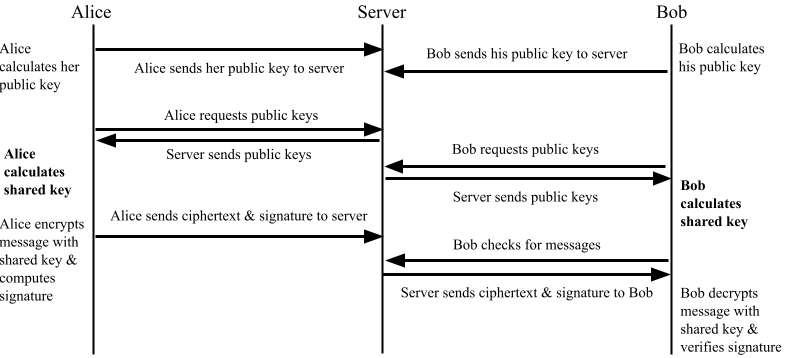
\includegraphics[width=\textwidth]{figures/Message Exchange Diagram.png}
    \caption{Message Exchange Diagram}
    \label{fig:messages}
\end{figure}

A message here can be either a text message or a file from Alice's device. 
The server stores a list of the public keys of every client who is connected, 
and will send this to any client who requests it in order for them to establish a shared key with other clients. 
The server also holds the encrypted data and the accompanying signature for messages which have yet to be requested by the recipient. 
After the recipient has asked the server if there are any messages waiting for them, the server has sent the relevant message(s), 
and the recipient has decrypted and verified the message(s), the server then deletes the message(s). 
The only data stored by the client is a list of their shared keys with other clients. 
As shown in Figure \ref{fig:messages}, all of the computation is done by the client and the server does not perform any calculations; 
it only receives, stores, and sends client data. 
There are two ECC specific algorithms performed by each client in the exchange shown in Figure \ref{fig:messages}, 
namely the Elliptic Curve Diffie-Hellman (ECDH) key exchange algorithm and the Elliptic Curve Digital Signature Algorithm (ECDSA). 

\subsection{Algorithms}\noindent \label{Algorithms}
This section outlines the algorithms which are used by my system and how I implemented them. 
The two ECC specific algorithms mentioned previously (ECDH and ECDSA) differ from their RSA counterparts (DH and DSA) only in that 
the operation of exponentiation of an integer is instead replaced by the operation of multiplying a point on an elliptic curve. 
The naive approach to this of repeatedly adding a point $G$ to itself $k$ times in order to calculate $kG$ would take prohibitively long. 
Therefore I had to implement an adapted version of the repeated squares method (squaring and multiplying integers) 
used by RSA to calculate large exponents efficiently. 
This adapted method I implement is to use doubling and adding of points on an elliptic curve in order to achieve multiplication of a point. 
While the naive approach would take $O(k)$ time to calculate $kG$, this approach takes $O(log(k))$ time, 
making it practical for my system since $k$ will be a very large number (of the order $2^{250}$). 
An elliptic curve (Section \ref{Elliptic Curve}), along with the operations of adding (Section \ref{Point Addition}) 
and doubling (Section \ref{Point Doubling}) points on the curve, are formally defined below. 

\subsubsection{Elliptic Curve}\noindent \label{Elliptic Curve}
Let $p$ be a prime number, and let $F_p$ denote the field of integers modulo $p$. 
An elliptic curve $E$ over $F_p$ is defined by an equation of the form:
\begin{equation}
y^2 = x^3 + ax + b,
\end{equation}

where $a,\, b \in F_p$ satisfy $4a^3 + 27b^2 \ne 0$ (mod $ p$).

\subsubsection{Point Addition}\noindent \label{Point Addition}
Let $P = (x_1,y_1) \in E(F_p)$ and $Q = (x_2,y_2) \in E(F_p)$, where $P \neq Q$. 
Then $P + Q = (x_3,y_3)$, where:
\begin{equation}
    x_3 = \lambda^2 - x_1 - x_2, \quad y_3 = \lambda(x_1 - x_3) - y_1, \quad and \quad \lambda = \frac{y_2-y_1}{x_2-x_1}.
\end{equation}

\subsubsection{Point Doubling}\noindent \label{Point Doubling}
Let $P = (x_1,y_1) \in E(F_p)$. 
Then $P + P = 2P = (x_3,y_3)$, where:
\begin{equation}
    x_3 = \lambda^2 - 2x_1, \quad y_3 = \lambda(x_1 - x_3) - y_1, \quad and \quad \lambda = \frac{3x_1^2 + a}{2y_1}
\end{equation}

\cite{hankerson2003guide,lopez2000overview}.

\vspace{5mm}

In my system when I want to multiply a point $G$ by an integer $k$, 
I take the point $G$ and double it $\lfloor log_2(k) \rfloor$ times, storing each new point in an array where index $i$ holds $2^i * G$. 
The final value is then calculated by adding the points in the array whose index corresponds to a $1$ in the binary expansion of $k$. 
My system actually implements this using bitwise operations on $k$ for efficiency, 
however it is more intuitive to imagine it as a binary expansion and an array of equal length as described. 
That is how I implement point multiplication using point addition and point doubling. 
Things are complicated further however due to the fact that an elliptic curve is defined over a field of integers modulo $p$ (\ref{Elliptic Curve}), 
meaning that these operations are all carried out in modulo $p$ and can only involve integers. 
Since the equations for both point addition (\ref{Point Addition}) and point doubling (\ref{Point Doubling}) involve division, 
it is clear that a naive implementation of division cannot be used here since it would produce non-integer results. 
Therefore I had to implement the Extended Euclidean algorithm (EEA) in order to ensure integer results of these division calculations. 
For example, in order to calculate the gradient $\lambda = \frac{y_2-y_1}{x_2-x_1}$ in point addition (\ref{Point Addition}), 
I use the EEA to calculate $(x_2-x_1)^{-1}$ mod $p$ and then multiply this by $(y_2-y_1)$. 
This ensures that $\lambda$ is an integer, and therefore that the coordinates $(x_3,y_3)$ as defined in \ref{Point Addition} 
are also integers. 

Once I had a function for efficiently computing point multiplication, I was able to move on to the functions of ECDH and ECDSA. 

\subsubsection{ECDH}\noindent \label{ECDH}
The \emph{Elliptic Curve Diffie-Hellman} key agreement protocol allows Alice and Bob 
to securely agree upon the value of a point on an elliptic curve, although neither of them initially knows the value of the point. 
This point becomes their shared key, and the algorithm for generating it is formally defined below. 


\subsubsection{Shared Key Establishment}\noindent
Alice and Bob must agree on a finite field $F_q$, an elliptic curve $E/F_q$, and a generator point $G \in E(F_q)$  of (prime) order $n$.
Both Alice and Bob have a key pair $(d,Q)$ consisting of a private key $d$ (a randomly selected integer less than $n$) 
and a public key $Q = d * G$.

\vspace{1mm}

0. \space Let $(d_A,Q_A)$ be the key pair of Alice and $(d_B,Q_B)$ be the key pair of Bob.

1. \space Alice computes $K = (x_K,y_K) = d_A * Q_B$

2. \space Bob computes $L = (x_L,y_L) = d_B * Q_A$

3. \space Since $d_AQ_B = d_Ad_BG = d_Bd_AG = d_BQ_A$. Therefore $K = L$ and hence $x_K = x_L$

4. \space Hence the shared secret is $x_K$

\vspace{1mm}

Since it is practically impossible to find the private key $d_A$ or $d_B$ from the public key $K$ or $L$, 
it is not possible for Eve to obtain the shared secret \cite{jurivsic1997elliptic,anoop2007elliptic,silverman2009arithmetic,brown2009standards}. 

\vspace{5mm}

In my implementation of this algorithm, all clients are automatically using the same generator point which lies 
on the same elliptic curve, defined over the same finite field. 
This is because every client is an instance of the same program and this is hard-coded. 
I generate the random private key for each client, using Python's "secrets" module, when the client instance is started. 
The public key is then calculated using the point multiplication function mentioned previously. 
This public key is sent to the server along with the user's name (e.g. Alice) which they have entered via the command line. 
Any other user (e.g. Bob) can then get Alice's public key from the server and establish a secret shared key with her. 
In my system, Bob (or any other client) calculates their shared key with Alice by first asking the server 
for any available public keys. 
Bob then uses the point multiplication function to multiply Alice's public key by his private key. 
The shared keys that each client has established with their contacts are stored locally 
and used to encrypt future messages with symmetric AES. 

\subsubsection{ECDSA}\noindent \label{ECDSA}
The \emph{Elliptic Curve Digital Signature Algorithm} allows Alice to sign a message or file in such a way that Bob is able to then 
verify that Alice must have been the sender and that the message/file has not been altered. 
Alice does this by generating a signature using the hash of the message and her private key. 
She then sends this to Bob alongside her message. 
Bob then uses Alice's public key and the hash of the message to check that the signature must have been generated on the same message and by Alice. 
The two parts of this algorithm are formally defined below. 

\subsubsection{Signature Generation}\noindent \label{Signature Generation}
For signing a message $m$ sent by Alice, using Alice's private key $d_A$.

\vspace{1mm}

1. \space Calculate $e = HASH(m)$, where $HASH$ is a cryptographic hash function, such as SHA

2. \space Select a random integer $k$ from $[1,n-1]$

3. \space Calculate $r = x1$, where $(x1,y1) = k * G$ (mod $n$)

4. \space Calculate $s = k^{-1}(e+d_Ar)$ (mod $n$)

5. \space The signature is the pair $(r,s)$

\subsubsection{Signature Verification}\noindent \label{Signature Verification}
For Bob to authenticate Alice's signature, Bob must have Alice's public key $Q_A$.

\vspace{1mm}

1. \space Calculate $e = HASH(m)$

2. \space Calculate $w = s^{-1}$ (mod $n$)

3. \space Calculate $u_1 = ew$ (mod $n$) and $u_2 = rw$ (mod $n$)

4. \space Calculate $(x_1,y_1) = u_1G + u_2Q_A$

5. \space The signature is valid if $x_1 = r$ (mod $n$), invalid otherwise

\vspace{2mm}

\cite{jurivsic1997elliptic,koblitz2000state,hankerson2003guide,anoop2007elliptic,silverman2009arithmetic,brown2009standards}.

\vspace{5mm}

In my implementation of this algorithm, Alice and Bob first agree upon all of the same initial setup things mentioned in Section \ref{ECDH} 
by default since again they are all hard-coded in to every client. 
When Alice wants to send a signed message or a file to Bob, she enters the message or the name of the file via the command line, 
and generates a hash of the message/file using SHA-512 from Python's "hashlib" module. 
This hash is converted to an integer and truncated to be smaller than $n$. 
A random number $k$ is then generated using the same "secrets" module previously mentioned and the point $G$ is multiplied by $k$ using 
the point multiplication function, with the x-coordinate taken as $r$ and the y-coordinate discarded. 
The integer $r$ is multiplied by Alice's private key (also an integer) and added to the truncated hash of the message (another integer), 
finally this is divided by $k$ to generate $s$. 
This division is done by multiplying by the inverse of $k$ modulo $n$, calculated with the EEA function mentioned earlier. 
Alice sends both $r$ and $s$ to the server, along with her AES encrypted message. 

On the receiving end of my implementation, after Bob receives all of this data from the server, 
he first decrypts the message itself using the shared key he has already established with Alice. 
He uses the plaintext message and the same hashing algorithm to generate a hash of the message, 
which he converts to an integer and truncates in the same way that Alice did, calling it $e$. 
The multiplicative inverse of $s$ modulo $n$ is then calculated using the EEA function and called $w$. 
Bob then does two integer multiplications, the first is the $e*w$ (mod $n$), 
and the second is $r*w$ (mod $n$), these new integers are called $u_1$ and $u_2$ respectively. 
Next, two lots of point multiplication are carried out and their results are summed by point addition. 
The first point multiplication is $u_1*G$ where $G$ is the generator point mentioned previously, 
and the second is $u_2*Q_A$ where the point $Q_A$ is Alice's public key. 
After adding these two points together using the point addition function to create a new point, 
Bob takes just the x-coordinate of this new point and compares it to the $r$ from Alice's signature. 
If these are equal (mod $n$) then the signature is valid and was definitely generated by Alice using the same message which Bob received. 
So now Bob has the plaintext message and is assured that it is authentic. 


\subsection{Tools used}\noindent \label{Tools}
The system was created entirely in Python. 
I chose this language because of both its ability to handle large integers with ease, 
and its large number of well-established modules for computing generic cryptographic functions. 
Since my system carries out operations involving huge integers, other less abstracted languages would 
have required much more involvement at the lower level which would only detract from my progress with the actual aims of the project. 
The specific Python modules that I used in my system are: "Pyro4", "AES" from "Cryptodome", "base64", "hashlib", "secrets", and "os". 
"Pyro4" is used for remote object invocation, "AES" for symmetric encryption, "base64" for decoding the AES ciphertext, 
and "hashlib" for generating hashes using SHA-2. 
I chose to use "secrets" because I realised that my initial implementation using "random" was not cryptographically secure. 
I used the "os" module for file management, since any files which the user receives are stored 
in a subdirectory labelled by their name. 
I only used long standing and well used libraries because of \cite{ducklin2021python}. 

The system can be started and interacted with via a command line interface. 
This was chosen since it allowed me to focus 
more on the protocols and back-end of the system rather than on designing a visually appealing graphical user interface (GUI). 
A GUI was not relevant to the mathematical-based aims of this project. 


\subsection{Implementation Issues}\noindent \label{Implementation}
After I successfully implemented client-client communication with separate instances of the client program running on the 
same machine, I then attempted to adapt the system for use with the client instances on separate machines on the same network. 
However, I encountered issues with this due to the security protocols in place on networks. 
I decided against attempting to circumvent these protocols due to both the potentially 
time-consuming nature of the problem and fact that my project is not aiming 
to recreate Signal or WhatsApp, network communication is not necessary. 


\subsection{Verification and Validation}\noindent \label{Verification}
This section will run through a real interaction between Alice and Bob using the system, 
specifically the exchange shown in Figure \ref{fig:messages}. 
This will demonstrate the calculations performed by the system and the validity of these calculations. 
All large numbers here are shown in hexadecimal, for brevity. 
This interaction uses an elliptic curve known as Curve25519 \cite{10.1007/11745853_14}, 
which can be expressed by the equation: 

\begin{equation}
    y^2 = x^3 + 486662x^2 + x \pmod{2^{255}-19}.
\end{equation}

This curve is most often expressed in the Montgomery \cite{montgomery1987speeding} form as above ($By^2 = x^3 + Ax^2 + x$), 
but can be converted to the more traditional short Weierstrass form shown earlier ($y^2 = x^3 + ax + b$) through substitution. 
Curve25519 has the base point $g = $ \\
({\footnotesize $0x9$}, {\footnotesize $0x20ae19a1b8a086b4e01edd2c7748d14c923d4d7e6d7c61b229e9c5a27eced3d9$}), \\
which has prime order $n = 2^{252} +$ {\footnotesize $0x14def9dea2f79cd65812631a5cf5d3ed$}. 
The curve's cofactor is $h = 8$. 


\subsubsection{Key Generation}\noindent
Alice's randomly generated private key is \\
{\footnotesize $0x69837a193b0f43bac8b32a30396a189c51706d49fcbb7c0e099b8f1b4bcb969$}. \\
When she multiplies the base point $g$ by this number, she obtains the point \\
({\footnotesize $0x67bf8995372ae1a9329f441d955193623aedf68a01ee5e2af7c33eabc27d9fd$}, \\
{\footnotesize $0xbc9a2fe41909056a46927d7c3af1ffed8e802854a32378df1845f819c016bdb$}) \\
as her public key.

Generated in the same way, Bob's private key is \\
{\footnotesize $0xf7d16d30314975879241ab2a17fdb1194fa2a7319b0b3331590c8482437f0b3$}. \\
Therefore his public key is \\
({\footnotesize $0x2ffeaa851900d44817e3888854d958a91b9e1127ed0057a2e6796f3a1115cda$}, \\
{\footnotesize $0x3fd4639dbd63076c19aeb51816711d7de4331cb75ec3c89ea1c387297660809c$}).


\subsubsection{Shared Key Establishment}\noindent
Alice calculates the shared key by $h \cdot d \cdot Q$, 
where $h$ is the cofactor, $d$ is Alice's private key, and $Q$ is Bob's public key. \\
Firstly, $d \cdot Q = $\\
({\footnotesize $0x7bb294204beba6ba902f5a21e14c4d5abc953d52b79be70377104f72de310a4a$}, \\
{\footnotesize $0x6d9d2ec13fc729a629259a1fcdf96d4a66e7e4e1365f54ed5fa56e235bc74b5$}) \\
Then multiplying by $h = 8$ gives $h \cdot d \cdot Q = $\\
({\footnotesize $0x37ae8d3aa1495b39ead29b8abe24e7d8d7f2fb05186216a37c4b55708ead1fd$}, \\
{\footnotesize $0x29aecf95ba814e3e52866f5daa243d3366e8c8d0255117ee047822319b44222c$}) \\
Therefore, Alice calculates the shared key as: 
\begin{equation} \label{AliceKey}
    0x37ae8d3aa1495b39ead29b8abe24e7d8d7f2fb05186216a37c4b55708ead1fd.
\end{equation}

Bob also calculates $h \cdot d \cdot Q$, except here $d$ is his private key and $Q$ is Alice's public key. 
$d \cdot Q = $ \\
({\footnotesize $0x7bb294204beba6ba902f5a21e14c4d5abc953d52b79be70377104f72de310a4a$}, \\
{\footnotesize $0x6d9d2ec13fc729a629259a1fcdf96d4a66e7e4e1365f54ed5fa56e235bc74b5$}) \\
Then multiplying by $h = 8$ gives $h \cdot d \cdot Q = $\\
({\footnotesize $0x37ae8d3aa1495b39ead29b8abe24e7d8d7f2fb05186216a37c4b55708ead1fd$}, \\
{\footnotesize $0x29aecf95ba814e3e52866f5daa243d3366e8c8d0255117ee047822319b44222c$}) \\
Bob's calculation of the shared key is: 
\begin{equation} \label{BobKey}
    0x37ae8d3aa1495b39ead29b8abe24e7d8d7f2fb05186216a37c4b55708ead1fd.
\end{equation}

This demonstrates that the ECDH part of the system works, since Alice and Bob each calculate the same shared key ( Key (\ref{AliceKey}) = Key (\ref{BobKey}) ). 
Critically, from a security perspective, only Alice and Bob can possibly know the value of this shared secret key 
because it was calculated using their respective private keys (which only they have access to). 
This makes it suitable for use as a symmetric AES key for end-to-end-encrypted communication between Alice and Bob. 


\subsubsection{Signature Generation}\noindent
The system allows Alice to send a message or file to Bob which is not only encrypted using the shared key that they have just established (through ECDH), 
but which is also digitally signed in such a way that Bob can verify the authenticity of the message. 
This subsection shows an example message sent by Alice to Bob, as in Figure \ref{fig:messages}. 

Alice wants to send the message ``Hello, Bob!" to Bob. 
Their shared key is converted from an integer to bytes, and used as an AES key to encrypt the message. 
The message is also hashed and then truncated to give the integer $e =$ \\
{\footnotesize $0x144b549f0522c7f6c224fe404e8200cfbe352c16883f16777d01ba8c81bce487$}. \\
Alice generates a random number $k$ and calculates $r = kG =$ 
\begin{equation}
    0xa96542405f3dc83b44e45beaa40d911efe8c5fee82a9f087cce28882b0fca82.
\end{equation}
Next, she calculates $s = k^{-1}(e + d \cdot r) =$ \\
{\footnotesize $0x237543088442522d4dfb6acb7126982df6d73473d1d89fe0d26f24226d79e82$}, where $d$ is her private key. \\
The signature that Alice sends, alongside the encrypted message, is the pair $(r,s)$. 

\subsubsection{Signature Verification}\noindent
When Bob receives the encrypted message and the signature pair $(r,s)$, 
he first uses the shared key (converted to bytes) to decrypt the message with AES. 
He then hashes the plaintext and truncates it to get the integer $e =$ \\
{\footnotesize$0x144b549f0522c7f6c224fe404e8200cfbe352c16883f16777d01ba8c81bce487$}. \\
Note that this is the same hash generated by Alice, but Bob doesn't yet know this since the hash itself is not sent. 
Alice calculates the x-coordinate of the point $v = (e \cdot s^{-1})G + (r \cdot s^{-1})Q =$ \\
\begin{equation}
    0xa96542405f3dc83b44e45beaa40d911efe8c5fee82a9f087cce28882b0fca82,
\end{equation}
where $Q$ is Alice's public key. 

Since this $v$ matches the $r$ in Alice's signature ($v=r$), 
Bob is assured that Alice sent the message, and that the content of the message is unchanged, 
since both Alice's private key, and the same hash must have been used to generate the signature. 




\subsubsection{Safe Curves}\noindent \label{Safe Curves}
There are several different standards covering selection of curves for use in elliptic-curve cryptography, 
most recently NSA Suite B (2005) and ANSSI FRP256V1 (2011). 
Each of these standards tries to ensure that the ECDLP (finding a user's private key, given their public key) is difficult. 
Unfortunately, there is a gap between ECDLP difficulty and ECC security. 
None of these standards do a good job of ensuring ECC security, 
secure implementations of the standard curves are theoretically possible but very hard. 
There are many attacks that break real-world ECC without solving ECDLP \cite{bernstein2013safecurves}. 
MORE DETAIL ABOUT WHAT MAKES A CURVE SAFE/UNSAFE

In 2006, Daniel Bernstein designed a new high-security ECDH function which achieved record setting speeds (twice as fast as any other function), 
with several side benefits including state-of-the-art timing-attack protection. 
This function, known as Curve25519, is suitable for a wide variety of cryptographic applications. 
The Curve25519 function is $F_p$-restricted x-coordinate scalar multiplication on $E(F_{p^2})$, 
where $p$ is the prime number $2^{255} - 19$ and $E$ is the elliptic curve $y^2 = x^3 + 486662x^2 + x$ \cite{10.1007/11745853_14}.
Curve25519 is regarded as a safe curve, since it satisfies the basic parameter requirements, the ECDLP security requirements, 
and the ECC security requirements beyond ECDLP security \cite{bernstein2013safecurves}.

\subsubsection{Exhaustive Search}\noindent \label{Exhaustive Search}
The elliptic curve parameters for cryptographic schemes should be carefully chosen in order to resist all known attacks on the ECDLP. 
The most na\"{\i}ve algorithm for solving the ECDLP is exhaustive search whereby one computes the sequence of points $P,2P,3P,4P,...$ until $Q$ is encountered. 
The running time is approximately $n$ steps in the worst case and $n/2$ steps on average. 
Therefore, exhaustive search can be circumvented by selecting elliptic curve parameters with $n$ sufficiently large to represent an infeasible amount of computation (e.g., $n \geq 2^{80}$) \cite{hankerson2003guide}.

\subsubsection{Pohlig-Hellman and Pollard's rho algorithm}\noindent \label{Pohlig-Hellman and Pollard's rho algorithm}
The best general-purpose attack known on the ECDLP is the combination of the Pohlig-Hellman algorithm and Pollard's rho algorithm, 
which has a fully-exponential running time of $O( \sqrt p \,)$ where $p$ is the largest prime divisor of $n$. 
To resist this attack, the elliptic curve parameters should be chosen so that $n$ is divisible by a prime number $p$ sufficiently large 
so that $\sqrt p$ steps is an infeasible amount of computation (e.g., $p > 2^{160}$).
If, in addition, the elliptic curve parameters are carefully chosen to defeat all other known attacks (e.g. Isomorphism attacks), 
then the ECDLP is believed to be infeasible given the state of today's computer technology \cite{hankerson2003guide}.

\subsection{Testing}\noindent \label{Testing}
Example of a working interaction


\section{Results}\noindent \label{Results}
This section presents the results of the solutions. 
It should include information on experimental settings. 
The results should demonstrate the claimed benefits/disadvantages of the proposed solutions.

This section should be between 2 to 3 pages in length.

- 25\% of paper

- Description of the evaluation method adopted - evaluated by trying to break the encryption and demonstrating that it would take an infeasible amount of time

- Clarity of results


Graphs from testing of security and efficiency of system: number of 1 bits vs time, log key value vs time, various curves vs time.

I analysed the time taken to compute $kG$ here and Figure \ref{fig:curves} shows the results. 
Add comparison with RSA timing, to make the comparison and have that data point for recommended size for security, 
draw vertical line saying this is the recommended size for good security for elliptic curves and it's taking 0.1 seconds, 
then have similar one for RSA at 2048 bits and hopefully it's longer

\begin{figure}[htb]
    \centering
    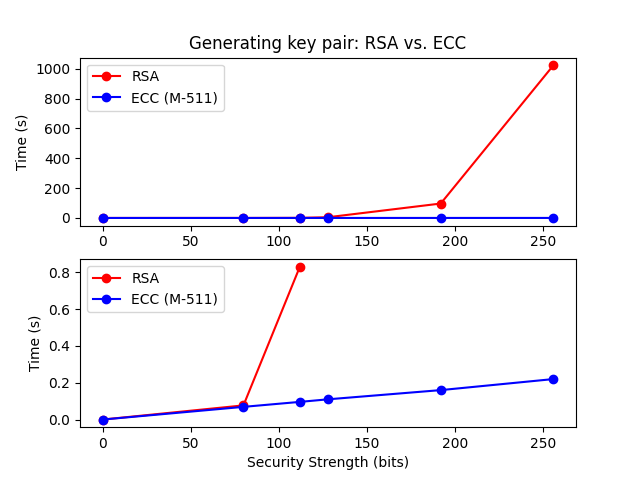
\includegraphics[width=0.4\textwidth]{figures/RSA.png}
    \caption{Comparison of RSA v ECC}
    \label{fig:rsa}
\end{figure}


\begin{figure}[htb]
    \centering
    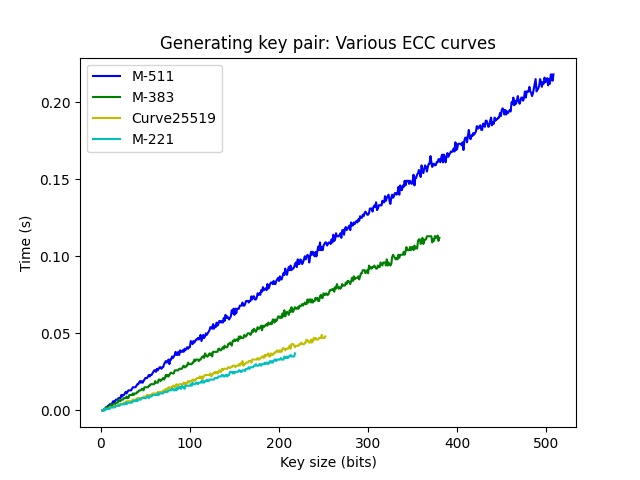
\includegraphics[width=0.4\textwidth]{figures/Timing.png}
    \caption{Comparison of various safe curves}
    \label{fig:curves}
\end{figure}

I also looked at whether my implementation leaks any information through timing attacks, 
for example, is it possible to determine how many 1s are in the binary expansion of the key by analysing the time taken to compute 
results in Figure \ref{fig:number1s}. 
\begin{figure}[htb]
    \centering
    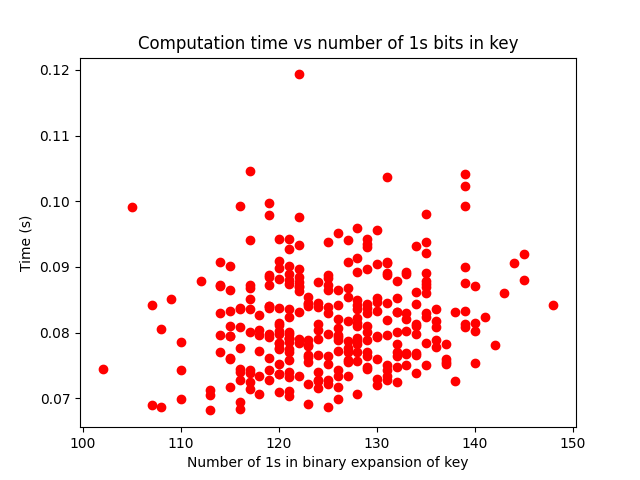
\includegraphics[width=0.4\textwidth]{figures/ones300SmoothedAny.png}
    \caption{Analysis of information leaked through timing attacks}
    \label{fig:number1s}
\end{figure}

I then investigated timing attacks with regards to the size of the binary expansion of the key in Figure \ref{fig:logbase2}

\begin{figure}[htb]
    \centering
    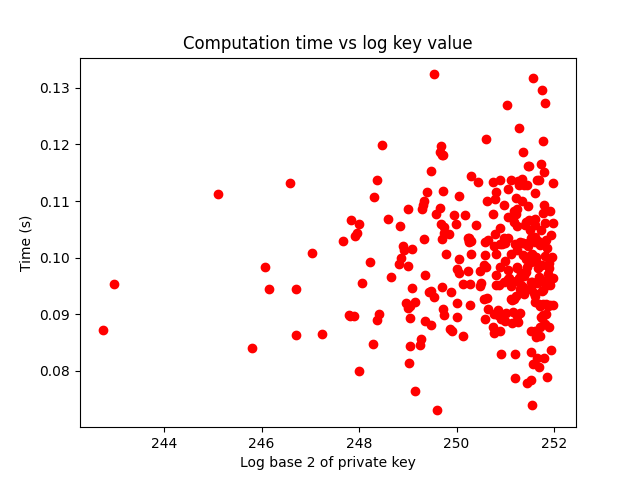
\includegraphics[width=0.4\textwidth]{figures/keyValue300SmoothedAny.png}
    \caption{Timing attacks analysis}
    \label{fig:logbase2}
\end{figure}



\section{Evaluation}\noindent
This section should between 1 to 2 pages in length.

- 20\% of paper

- Suitability of approach

- Discussion of strengths and limitations of the system - limitations with communicating over networks, works well with multiple client instances on a local machine

- Discussion of algorithms used - ECDH, ECDSA, point addition and point multiplication

- Appraisal of project organisation


\section{Conclusions}\noindent
This section summarises the main points of this paper. 
Do not replicate the abstract as the conclusion. 
A conclusion might elaborate on the importance of the work or suggest applications and extensions. 
This section should be no more than 1 page in length. 

- 5\% of paper

- Description of the main findings

- Clarity of conclusions

- Discussion of further work

Much research has been done into Elliptic Curve Cryptography since its discovery in 1985 \cite{10.1007/3-540-39799-X_31,koblitz1987elliptic}. 
The security of ECC is based on the hardness of the ECDLP, 
and currently the best algorithms known to solve the ECDLP have fully exponential running time. 
In contrast to the subexponential-time algorithms known for the integer factorisation problem, 
on which the security of RSA is based. 
This means that, for example, a 160-bit EC key provides the same level of security as a 1024-bit RSA key \cite{hankerson2003guide,silverman2009arithmetic}. 
ECC is a very strong encryption method, but only when implemented properly, 
using a safe curve \cite{bernstein2013safecurves,10.1007/11745853_14}
and a good random number generator \cite{hotz2010console}. 


\bibliography{projectpaper}


\end{document}
